\chapter{Background}

This chapter concludes the fundamental knowledge that is needed to comprehend the upcoming practical work. Firstly, an introduction to cloud computing will be held. Next, a throrough understanding of honeypots is given. Lastly, we introduce some concepts of intrusion detection systens.

\section{Virtualization}

\subsection{Docker}

\section{Cloud Computing}\todo{Check cites}

Nowadays it is one of the well-known keywords and has been used by vary large companies such as Google, or Amazon, however, the term \enquote{cloud computing} dates back to the late 1996, when a small group of technology executives of Compaq Computer framed new business ideas around the Internet.\cite{regalado2020} Starting from 2007 cloud computing evolved into a serious competitor and outnumbered the keywords \enquote{virtualization}, and \enquote{grid computing} reported by Google trends \cite{Wang2010}. Shortly, various cloud provider become publicly available, each with their own strengths and weaknesses. For example IBM's Cloud\footnote{\url{https://www.ibm.com/cloud}}, Amazon Web Services\footnote{\url{https://aws.amazon.com/}}, and Google Cloud\footnote{\url{https://cloud.google.com/}}. Why are clouds so attractive in practice?

\begin{itemize}
    \item It offers major advantages in terms of cost and reliability. When demand is needed, consumers do not have to invest in hardware when launching new services. Pay-as-you-go allows flexibility.
    \item Consumer can easily scale with demand. When more computational resources are required due to more requests, scaling up instances in conjunction with a suited price model are straightforward.
    \item Geographically distributed capabilities supply the need for world-wide scattered services.
\end{itemize}

In this section, we want to give basic unterstandings of cloud computing. First, we exhibit the history and draw some motivation. Following, we look at some the definitions, and point out characteristics. Lastly, we give an short introduction to HeiCloud, a cloud service that is offered by Heidelberg University.

\subsection{Definition of Cloud Computing}

Considering the definition of Brian Hayes, cloud computing is \enquote{a shift in the geography of computation} \cite{hayes2008}. Thus, computational workload is moved away from local instances towards services and datacenters that provide the need of users \cite{Armbrust2010}.

Considering the definition of the \ac{nist}, cloud computing \enquote{is a model for enabling ubiquitous, convenient, on-demand network access to a shared pool of configurable computing resources (e.g., networks, servers, storage, applications, and services) that can be rapidly provisioned and released with minimal management effort or service provider interaction} \cite{Mell2011}. \ac{nist} not only reflects the geographical shift of resources such as datacenters, but also mentions on-demand usage that contributes to a flexible resource management. Morever, \ac{nist} composes the term in five essential characteristics, three service models (see \autoref{subsec:cloud-service}), and four deployment models (see \autoref{subsec:cloud-deployment}) \cite{Mell2011}:\\

\textit{On-demand-self-service} refers to the unilaterally provision computing capabilities. Consumers can acquire server time and network storage on demand without a human interaction.\\

\textit{Broad network access} characterizes the access of capabilities of the network through standard protocols such as \ac{http}. Heterogeneous thin and thick client platforms should be supported.\\

\textit{Resource pooling} allows the provider's computing resources to be pooled across several consumers. A multi-tanent model with different physical and virtual resources are assigned on demand. Other aspects such as location are independent and cannot be controlled on a low-level by consumers. Moreover, high-level access to specify continent, state, or datacenter can be available.\\

\textit{Rapid elasticity} offers consumers to extend and release capabilities easily. Further automization to quickly increase resources  when demand skyrockets significantly can be supported regardless limit and quantity at any time.\\

\textit{Measured service} handles resources in an automated and optimized manner. It uses additional metering capabilities to trace storage, processing, bandwith, and active user accounts. This helps to monitor, and control resource usage. Thus, contributing to transparency between provider and consumer.

\subsection{Service models}
\label{subsec:cloud-service}

Service models are categorized by \ac{nist} into three basic models based on usage and abstraction level. \autoref{fig:cloud-functionalities}\todo{Fix image} shows the connection between each model whereas cloud resource are defined in \autoref{subsec:cloud-deployment}. Due to vast range of functionalities, \ac*{iaas} builds the foundation of service models. Each model on top represents a user-friendly abstraction with derated capabilities. \autoref{tab:example-service-models} shows examples of such service models.

\begin{figure}[h]
    \centering
    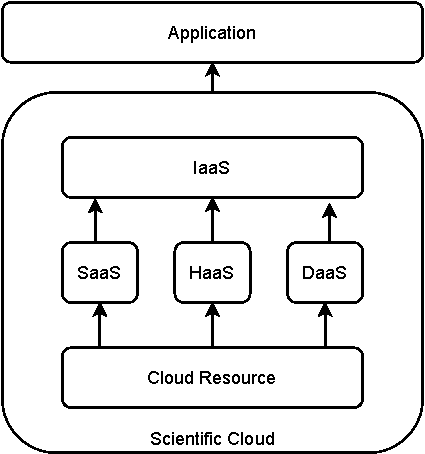
\includegraphics[width=0.4\textwidth]{figures/cloud-functionalities.pdf}
    \caption{Cloud functionalities (derived from \cite{Wang2010})}
    \label{fig:cloud-functionalities}
\end{figure}

\ac{saas} is a high-level abstraction to consumers. Controlling the underlying infrastructure is not supported. Often provider uses a multi-tenancy system architecture to organize each consumer's application in a separate environment. It helps to employ scaling with respect to speed, security availability, disaster recovery, and maintenance. Main objective of \ac{saas} is to host consumer's software or application that can be accessed over the Internet using either a thin or rich client.\cite{Dillon2010} \enquote{Limited user-specific application configuration settings} can be made \cite{Mell2011}.\\

\ac{paas} pivots on the full \enquote{Software Lifecycle} of an application whereas \ac{saas} distincts on hosting complete applications. \ac{paas} offers ongoing development and includes programming environment, tools, configuration management, and other services. In addition, the underlying infrastructure is not managed by the consumer.\\

\ac{iaas} offers a low-level abstraction to consumers with the ability to run arbitrary software regardless of operating system or application. In contrast to \ac{saas}, IT infrastructures capabilities (such as storage, networks) can be used. It strongly depends on virtualization due to integration, or decomposition of physical resources. \\

\ac{daas} serves as a virtualized data storage service on demand. Motivations behind such services could be upfront costs of on-premise enterprise database systems.\cite{Dillon2010} Mostly they require \enquote{dedicated server, software license, post-delivery services, and in-house IT maintenance} \cite{Dillon2010}. Whereas \ac{daas} costs solely what consumer's need.When dealing with a tremendous amount of data, file systems and RDBMS often lack in performance. \ac{daas} outruns such weak links by employing a table-style abstraction that can be scaled.\cite{Dillon2010}\\

\ac{haas} offers IT hardware, or datacenters to buy as a pay-as-you-go subscription service. The term dates back to 2006 during a time when hardware virtualization became more powerful. It is flexible, scalable and manageable.\cite{Wang2010}\\

\begin{table}[h]
    \centering
    \caption{Examples for cloud service models}
    \begin{tabularx}{\linewidth}{X|X|X|X|X}
        SaaS            & PaaS                  & IaaS       & Daas             & HaaS       \\ \hline
        Google Mail     & Google App Engine     & HeiCloud   & Adobe Buzzword   & Amazon EC2 \\
        Google Docs     & Windows Azure         & Amazon EC2 & ElasticDrive     & Nimbus     \\
        Microsoft Drive & AWS Elastic Beanstalk &            & Google Big Table & Enomalism  \\
                        &                       &            & Amazon S3        & Eucalyptus \\
                        &                       &            & Apache HBase     &            \\
    \end{tabularx}
    \label{tab:example-service-models}
\end{table}

\subsection{Deployment models}
\label{subsec:cloud-deployment}

Deployment models are categorized by \ac{nist} into four basic models. Each differs in data privacy, location, and manageablility \cite{Mell2011}. \autoref{tab:example-deployment-models} shows examples of such deployment models.

\begin{table}[h]
    \centering
    \caption{Examples for cloud deployment models}
    \begin{tabular}{l|l|l|l}
        Private Cloud & Community Cloud & Hybrid Cloud & Public Cloud     \\ \hline
                      & Seafile         &              & Amazon EC2       \\
                      & Nextcloud       &              & Google AppEngine \\
    \end{tabular}
    \label{tab:example-deployment-models}
\end{table}

Private clouds offer the highest level of control in regard of data privacy, and utilization. Mostly, such clouds are deployed within in a single organization, either managed by in-house teams or third party suppliers. In addition, it can be on or off premise. Within private clouds consumers have full control of their data. Especially for European data privacy laws, it is not negligible when data is stored abroad and thus under law of foreign countries. However, the popularity has not been withdrawn due to immense costs when moving towards public clouds. \cite{Dillon2010} \cite{Mell2011}\\

Community clouds can be seen as a conglomerate of mutliple organizations that merge their infrastructure with respect to a commonly defined policy, terms, and condition beforehand.\\

Public clouds represents the most used deployment models. In contradiction to private one, public clouds are fully owned by the service provider such as business, academics, or government organization. Consumers do not know where their data is distributed. In addition, contracts underlie custom policies.\\

Hybrid cloud is a mixure of two or more cloud infrastructures, such as private and public cloud.However, each entity keeps its core element. However, hybrid clouds defines \enquote{standardized or propriertary technology to enables data and application portability}\cite{Mell2011}.\\

%\subsection{Cloud Security}

%\cite{Nithin2012}

\subsection{HeiCloud}

\ac{iaas}\todo{Get information or paper about that}

\section{Honeypots}

The term \enquote{honeypot} exists since more than a decade. 1997 was the first time that a free honeypot solution became public. \ac{dtk}, developed by Fred Cohen, released the first honeypot solution. However, the earliest drafts of honeypots are from 1990/91, and built the foundation for Fred Cohen's \ac*{dtk}. Clifford Stoll's book \textit{The Cuckoo's Egg}, and Bill Cheswick's whitepaper \textit{En Evening With Berferd} describe concepts that are consider nowadays as honeypots. \cite{Spitzner2003}

\subsection{Definition of a Honeypot}

Dozen of defintions for honeypots circulate through the web. Thus, to cope with all the subtle differences, we want to exhibit some of the definitions and narrow down a common one.

Spitzner defines honeypots as a \enquote{security resource whose value lies in being probed, attacked, or compromised.}\cite{Spitzner2003}

\begin{enumerate}
    \item Low-interaction honeypots
    \item Medium-interaction honeypots
    \item High-interaction honeypots
\end{enumerate}

\subsection{Classification of Honeypots}

Low-interaction honeypots\\

Medium-interaction honeypots\\

High-interaction honeypots\\

Pure honeypots\\

%\subsection{Honeyd}

%\subsection{Configuration Honeyd}

\subsection{Value of Honeypots}

\subsection{Honeynets}

\cite{Spitzner2003}

\subsection{Legal Issues}

\cite{Spitzner2003}

\section{Summary}

